\documentclass{standalone}
\usepackage{tikz}
\begin{document}
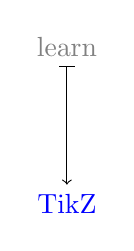
\begin{tikzpicture}

\node[gray] (A) at (0,2) {learn};
\node[blue] (B) at (0,0) {TikZ};
\draw[|->]  (A) -- (B);

\end{tikzpicture}
\end{document}
